\chapter{Máy đo chức năng hô hấp để bàn SpiroScout}
\section{Giới thiệu chung}
Máy đo chức năng hô hấp SpiroScout là hệ thống phế dung kế (Spirometer) hiện đại, được sản xuất bởi hãng Ganshorn, thương hiệu hàng đầu thế giới về công nghệ chuẩn đoán chức năng phổi. Khác với các dòng máy truyền thống sử dụng tuabin hay cảm biến chênh áp, SpiroScout nổi bật nhờ ứng dụng công nghệ đo lượng bằng sóng siêu âm. Công nghệ này cho phép đo trực tiếp lưu lượng và thể tích khí mà không gây ra sức cản hô hấp cho bệnh nhân, đồng thời loại bỏ các sai số do quán tính cơ học hay ngưng tụ hơi nước.\\
Thiết bị đáp ứng đầy đủ các tiêu chuẩn quản lý chất lượng và an toàn y tế quốc tế khắt khe như ISO 13485, FDA, CE.
\section{Tiêu chuẩn an toàn}

\subsection{Mục đích sử dụng}
Máy đo chức năng hô hấp cùng phần mềm LFX là một hệ thống siêu âm dựa trên PC để đo và phân tích lưu lượng và thể tích hơi thở, các thông số chức năng phổi ở bệnh nhân người lớn và trẻ em trên 5 tuổi.
Được chỉ định trong các trường hợp sau: \cite{manual_Spiroscout}
\begin{itemize}
    \item Để phát hiện sự hiện diện hay vắng mặt của rối loạn chức năng phổi
    \item Để xác định ảnh hưởng của bệnh phổi.
    \item Sàng lọc các cá nhân có nguy cơ mắc bệnh phổi.
    \item Để đánh giá rủi ro trước phẫu thuật.
    \item Để đánh giá các tác động tiềm ẩn hoặc phản ứng với môi trường hoặc nghề nghiệp phơi bày.
    \item Để đánh giá sự suy yếu và khuyết tật
    \item Theo dõi tác dụng của điều trị
    \item Mô tả diễn biến của bệnh phổi
\end{itemize}

\subsection{Chống chỉ định}
Việc sử dụng SpiroScout với phần mềm LFX không được chỉ định cho các trường hợp sau: \cite{manual_Spiroscout}
\begin{itemize}
    \item Ho ra máu không rõ nguồn gốc
    \item Tình trạng tim mạch không ổn định.
    \item Phình động mạch ngực, bụng hoặc não.
    \item Có bất kỳ bệnh cản trở nào có thể ảnh hưởng đến hiệu suất xét nghiệm
    \item Đau ngực hoặc bụng vì bất kỳ nguyên nhân nào
    \item Đau miệng hoặc mặt trầm trọng hơn do động ngãm hoặc các phẫu thuật gần đây khác
    \item Mới phẫu thuật ngực hoặc bụng
    \item Tiểu không tự chủ khi gắng sức
    \item Sa sút trí tuệ hoặc trạng thái lú lẫn
    \item Trẻ em dưới 5 tuổi.
\end{itemize}


\section{Cấu tạo và thông số kỹ thuật}
Danh sách các bộ phận: \cite{manual_Spiroscout}
\begin{itemize}
    \item Máy tính để bàn tích hợp phần mềm LFX
    \item SpiroScout với phần mềm LFX
    \item Bộ phận cơ sở và cảm biến SpiroScout
    \item Cáp cảm biến Spiro( cảm biến tới bộ phận đế)
    \item Cáp USB máy tính
    \item Bộ lọc PFT
\end{itemize}

\subsection{Máy tính trạm}

\begin{figure}[H]
    \centering
    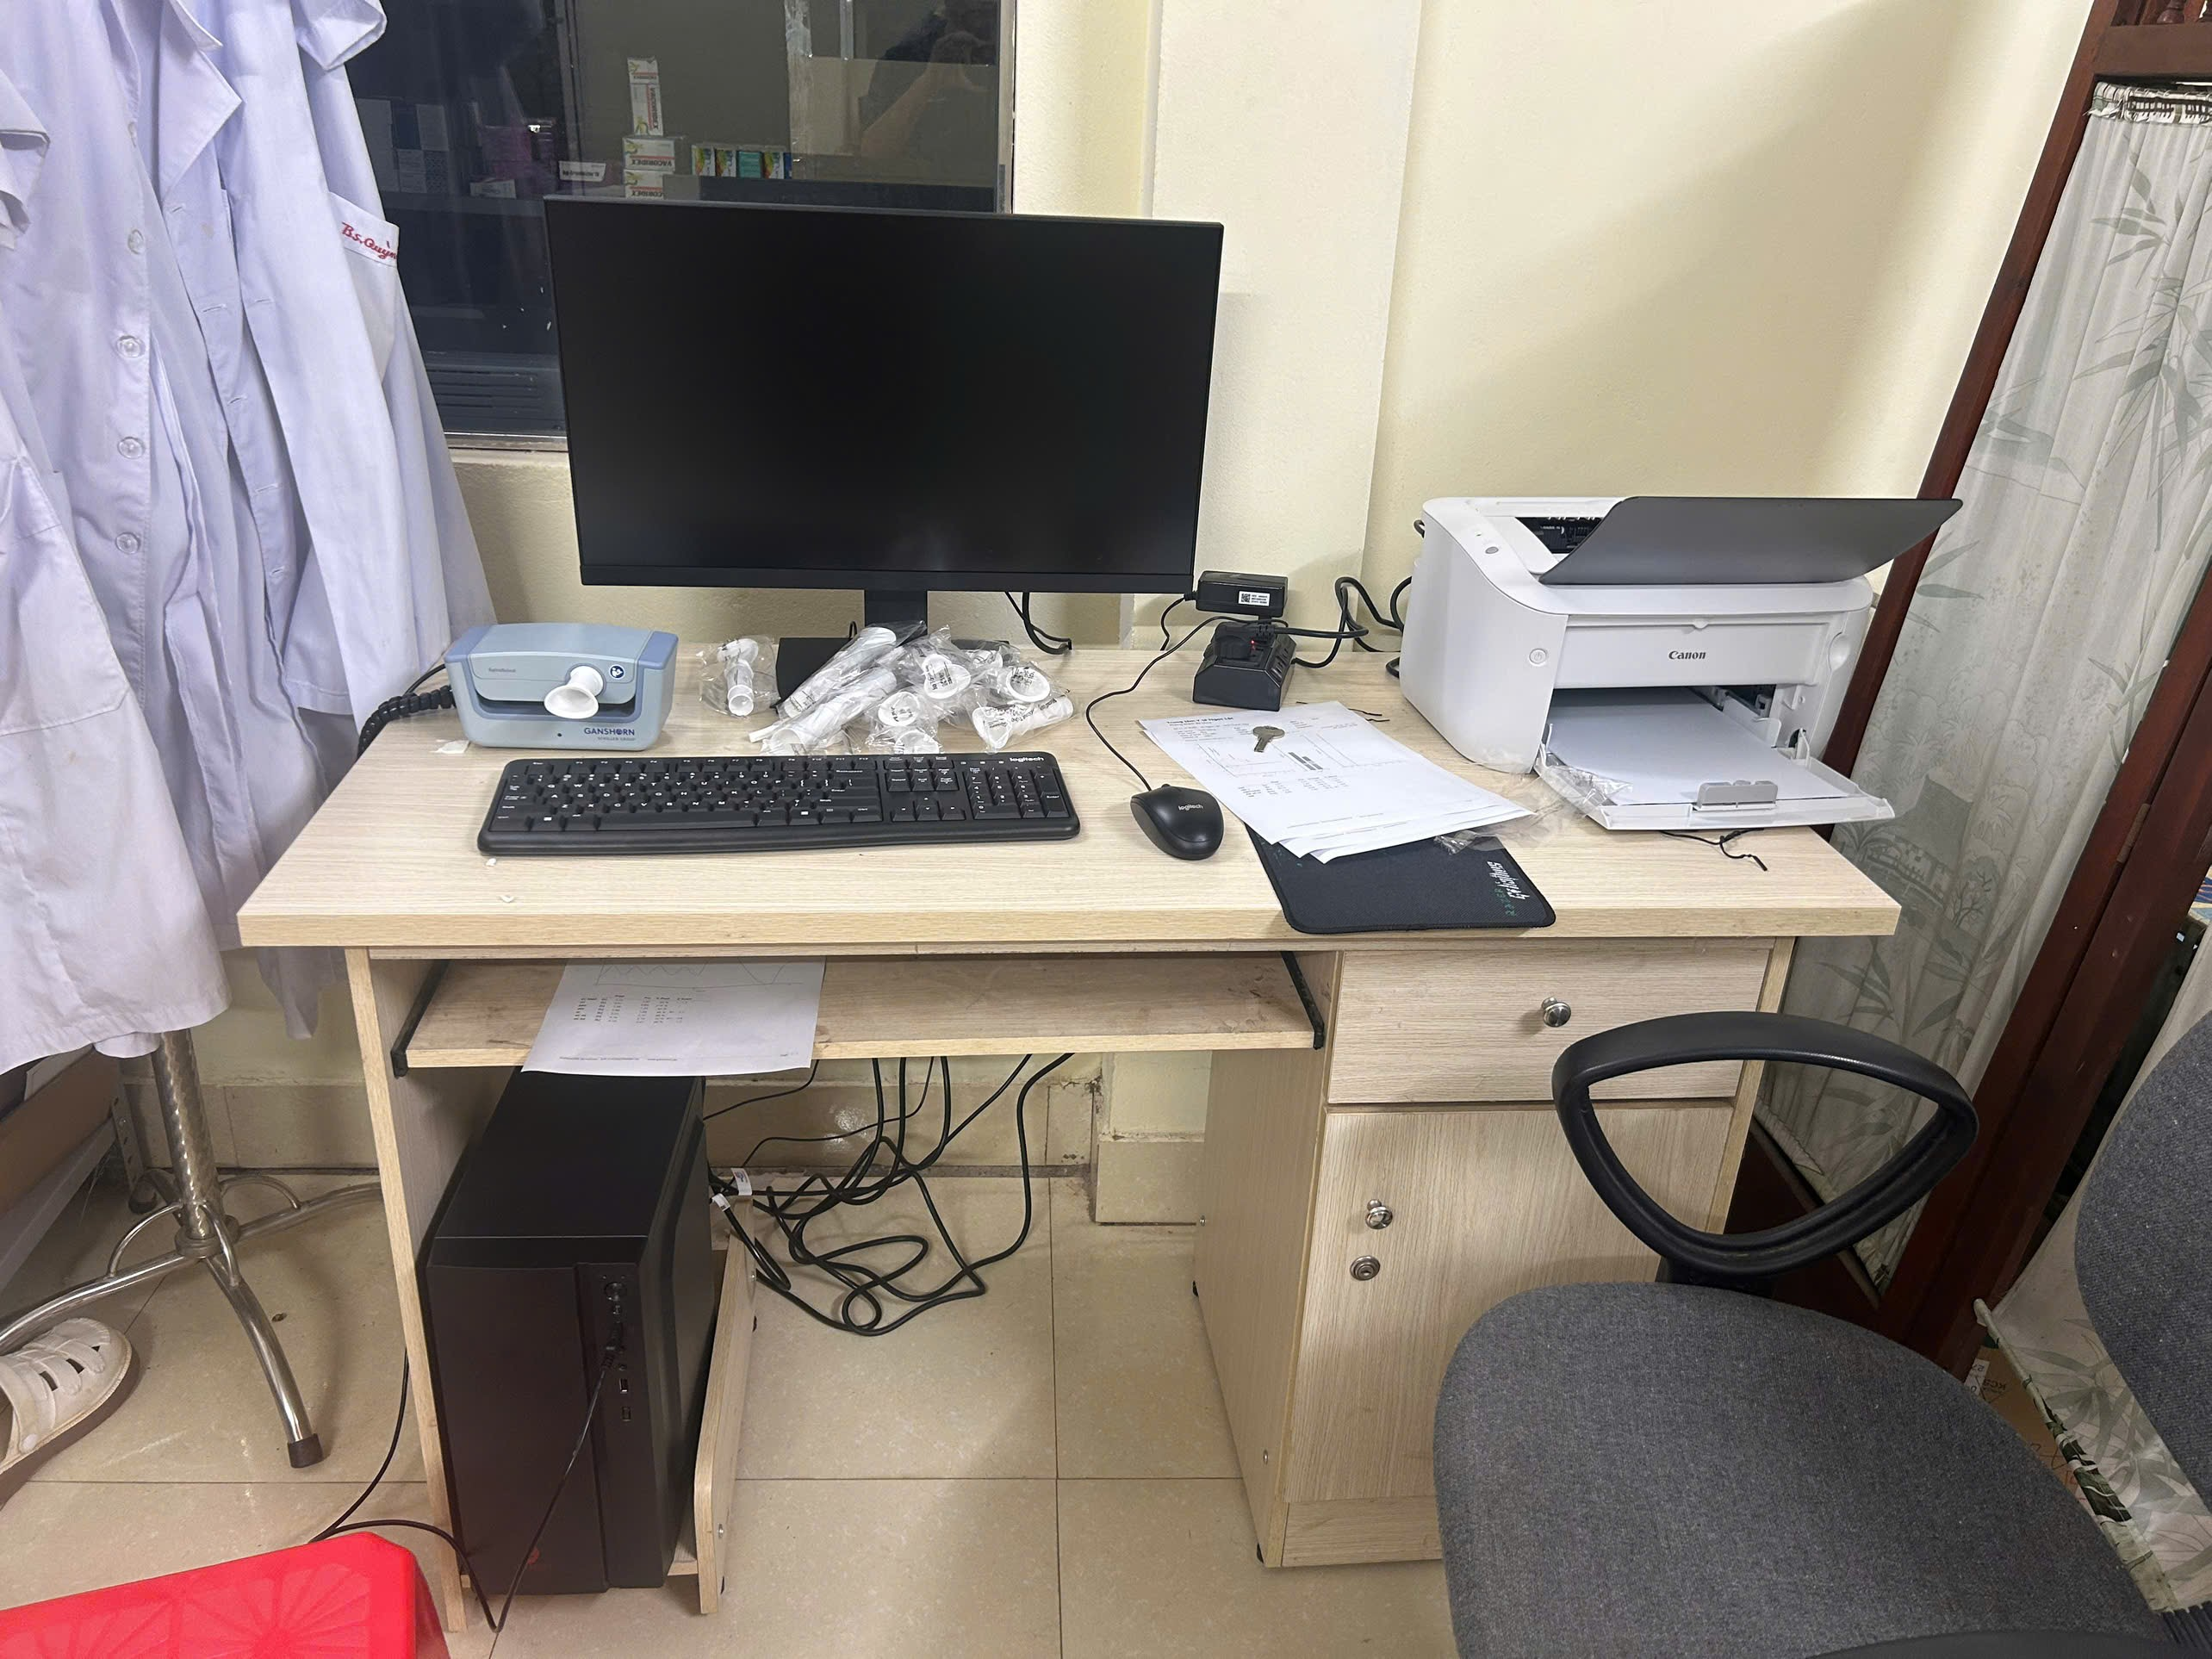
\includegraphics[width=0.5\linewidth]{PC-system.png}
    \caption{Hình ảnh thực tế máy tính trạm ở Trung tâm Y Tế Huyện Ngọc Lặc - Thanh Hoá - Việt Nam}
    \label{fig:placeholder}
\end{figure}

\begin{tabular}{ll}
    \toprule
    Thông số kỹ thuật của PC & \\
    \midrule
    An toàn    & Tuân thủ tiêu chuẩn IEC 60950-1 \\
     Hệ thống vận hành & Windows 7 Professional, 64-bit hoặc 32-bit\\
     Bộ xử lý  & Bộ xử lý tương thích Intel Core i5, 4.0 GHz\\
     Hiệu năng & 1.0 (4.0)\\
     RAM & 4 GB \\
     Bộ nhớ & 5 GB\\
     Độ phân giải màn hình & 1248 x 728\\
     Giao tiếp & USB \\
     \bottomrule
\end{tabular}

\subsection{Phần mềm LPX}

\begin{tabular}{ll}
    \toprule
    %Thông số kỹ thuật phần mềm cho Windows 32 hoặc 64 bit \\
    %\midrule
    Phân loại &  \\
    \midrule
    Thiết bị & Thiết bị y tế chủ động, loại IIa\\
    Phần ứng dụng & Type BF \\
    \midrule
    Hiệu chỉnh & \\
    \midrule
    F/V & ERS hoặc ATS \\
    Hít vào (Inhalation) & BTPS (modun môi trường) hoặc hiệu chỉnh BTPS thời gian thực \\
    Thể tích khí & STPD ( modun môi trường ) hoặc hiệu chỉnh BTPS thời gian thực \\
    \midrule
    Kết nối máy tính\\
    \midrule
    Dữ liệu tới PC & USB 2.0\\
    USB kết nối & Đầu nối A–đầu nối B / dây đôi bọc chống nhiễu / 2 x AWG24,  2 x AWG28\\
    Truyền tín hiệu & Cách ly quang 4 kV RS232, 57.600 Baud\\
    \midrule
    Dữ liệu\\
    \midrule
    Local & Ganshorn SQL\\
     & Xác thực do người dùng định nghĩa \\
     GDT & Nhập và xuất với các cài đặt do người dùng định nghĩa\\
     SEMA3 & tích hợp SCHILLER SEMA3\\
     \midrule
     Đo lưu lượng\\
     \midrule
     Nguyên lý đo & Đo thời gian truyền sóng siêu âm\\
     Khoảng đo & 0 đến +20 l/s\\
     Độ chính xác & < ±2 \% \\
     Độ phân giải & 1 ml \\
     \midrule
     Giá trị đo & \\
     \midrule
      & FEV 1 [L] \\
       & ... \\
    \bottomrule
    
\end{tabular}

\subsection{SpiroScout}

\begin{figure}[H]
    \centering
    \includegraphics[width=0.5\linewidth]{Kích-thước-tổng-quát.png}
    \caption{General dimension}
    \label{fig:placeholder}
\end{figure}

\begin{itemize}
    \item Cảm biến Scout cầm tay với bộ lọc thở dùng một lần: ScoutSensor cầm tay có một miếng đệm thở dùng một lần có thể tháo rời. Trong một số trường hợp lắp đặt, bộ lọc vi khuẩn xài một lần được sử dụng bộ chuyển đổi hình tròn khác.
    \item Base station: Trạm cơ sở cung cấp nền tảng an toàn cho SpiroScout khi không sử dụng và cũng được trang bị hệ thống điều khiển điện tử và các cảm biến để đo điều kiện môi trường xung quanh.
\end{itemize}
\begin{figure}[H]
    \centering
    \includegraphics[width=0.5\linewidth]{SpiroScout.png}
    \caption{SpiroScout}
    \label{fig:placeholder}
\end{figure}

\begin{tabular}{ll}
\toprule
    Thông số kỹ thuật của cảm biến SpiroScout\\
    \midrule
    General &  \\
    \midrule
    Kích thước & 18 cm x 9 cm x (W x H x D)\\
    \addlinespace
    Cân nặng & 1000g (ScoutSensor 185g, Trạm cơ sở 730g, dây 85g)\\
    \addlinespace
    Trở kháng hô hấp & 0.02 kPa/l/s = xấp sỉ 0.02 cmH20/l/s\\
    \addlinespace
    Dead space, complete & 18 cm3\\
    \addlinespace
    Chất liệu & Polythylene\\
    \midrule
    Bảo vệ và vệ sinh bệnh nhân & Chỉ dùng cho bệnh nhân, dùng một lần \\
         & Ống thở SpiroScout, Spirette™ với ống ngậm định hình công thái học và chóp tiêu chuẩn 22 mm, hoặc\\
         &  Bộ lọc vi khuẩn PFT GANSHORN\\
    \midrule
    Nguồn cấp & \\
    \midrule
    Tiêu chuẩn & Cấp nguồn qua USB 2.0 \\
     & Điện áp 4.5 đến 5.25 V DC\\
     & Dòng: 500 mA\\
     \midrule
     Cài đặt nguồn & Bộ đổi nguồn AC bên ngoài \\
     \midrule
     Thông số kỹ thuật của bộ đổi nguồn AC & EGSTON P2CFMW 6 Watt, 5 VDC\\
      & Đầu nối phụ MP205 (tiêu chuẩn y tế). Tiếp điểm bên trong = nối đất, ngoài =+5 VDC,\\
       & Protection class II\\
        & Phạm vi điện áp 100 đến 240 V, 50 đến 60 Hz,\\
    \midrule
    Sự tiêu thụ năng lượng & Chế độ chờ: 275 mA, 5 VDC (1.4 W),\\
     & Chế độ đo: 500mA, 5 VDC (2.5 W)\\
    \bottomrule
\end{tabular}
\subsection{ScoutTube - FPT Filter}

\begin{figure}[H]
    \centering
    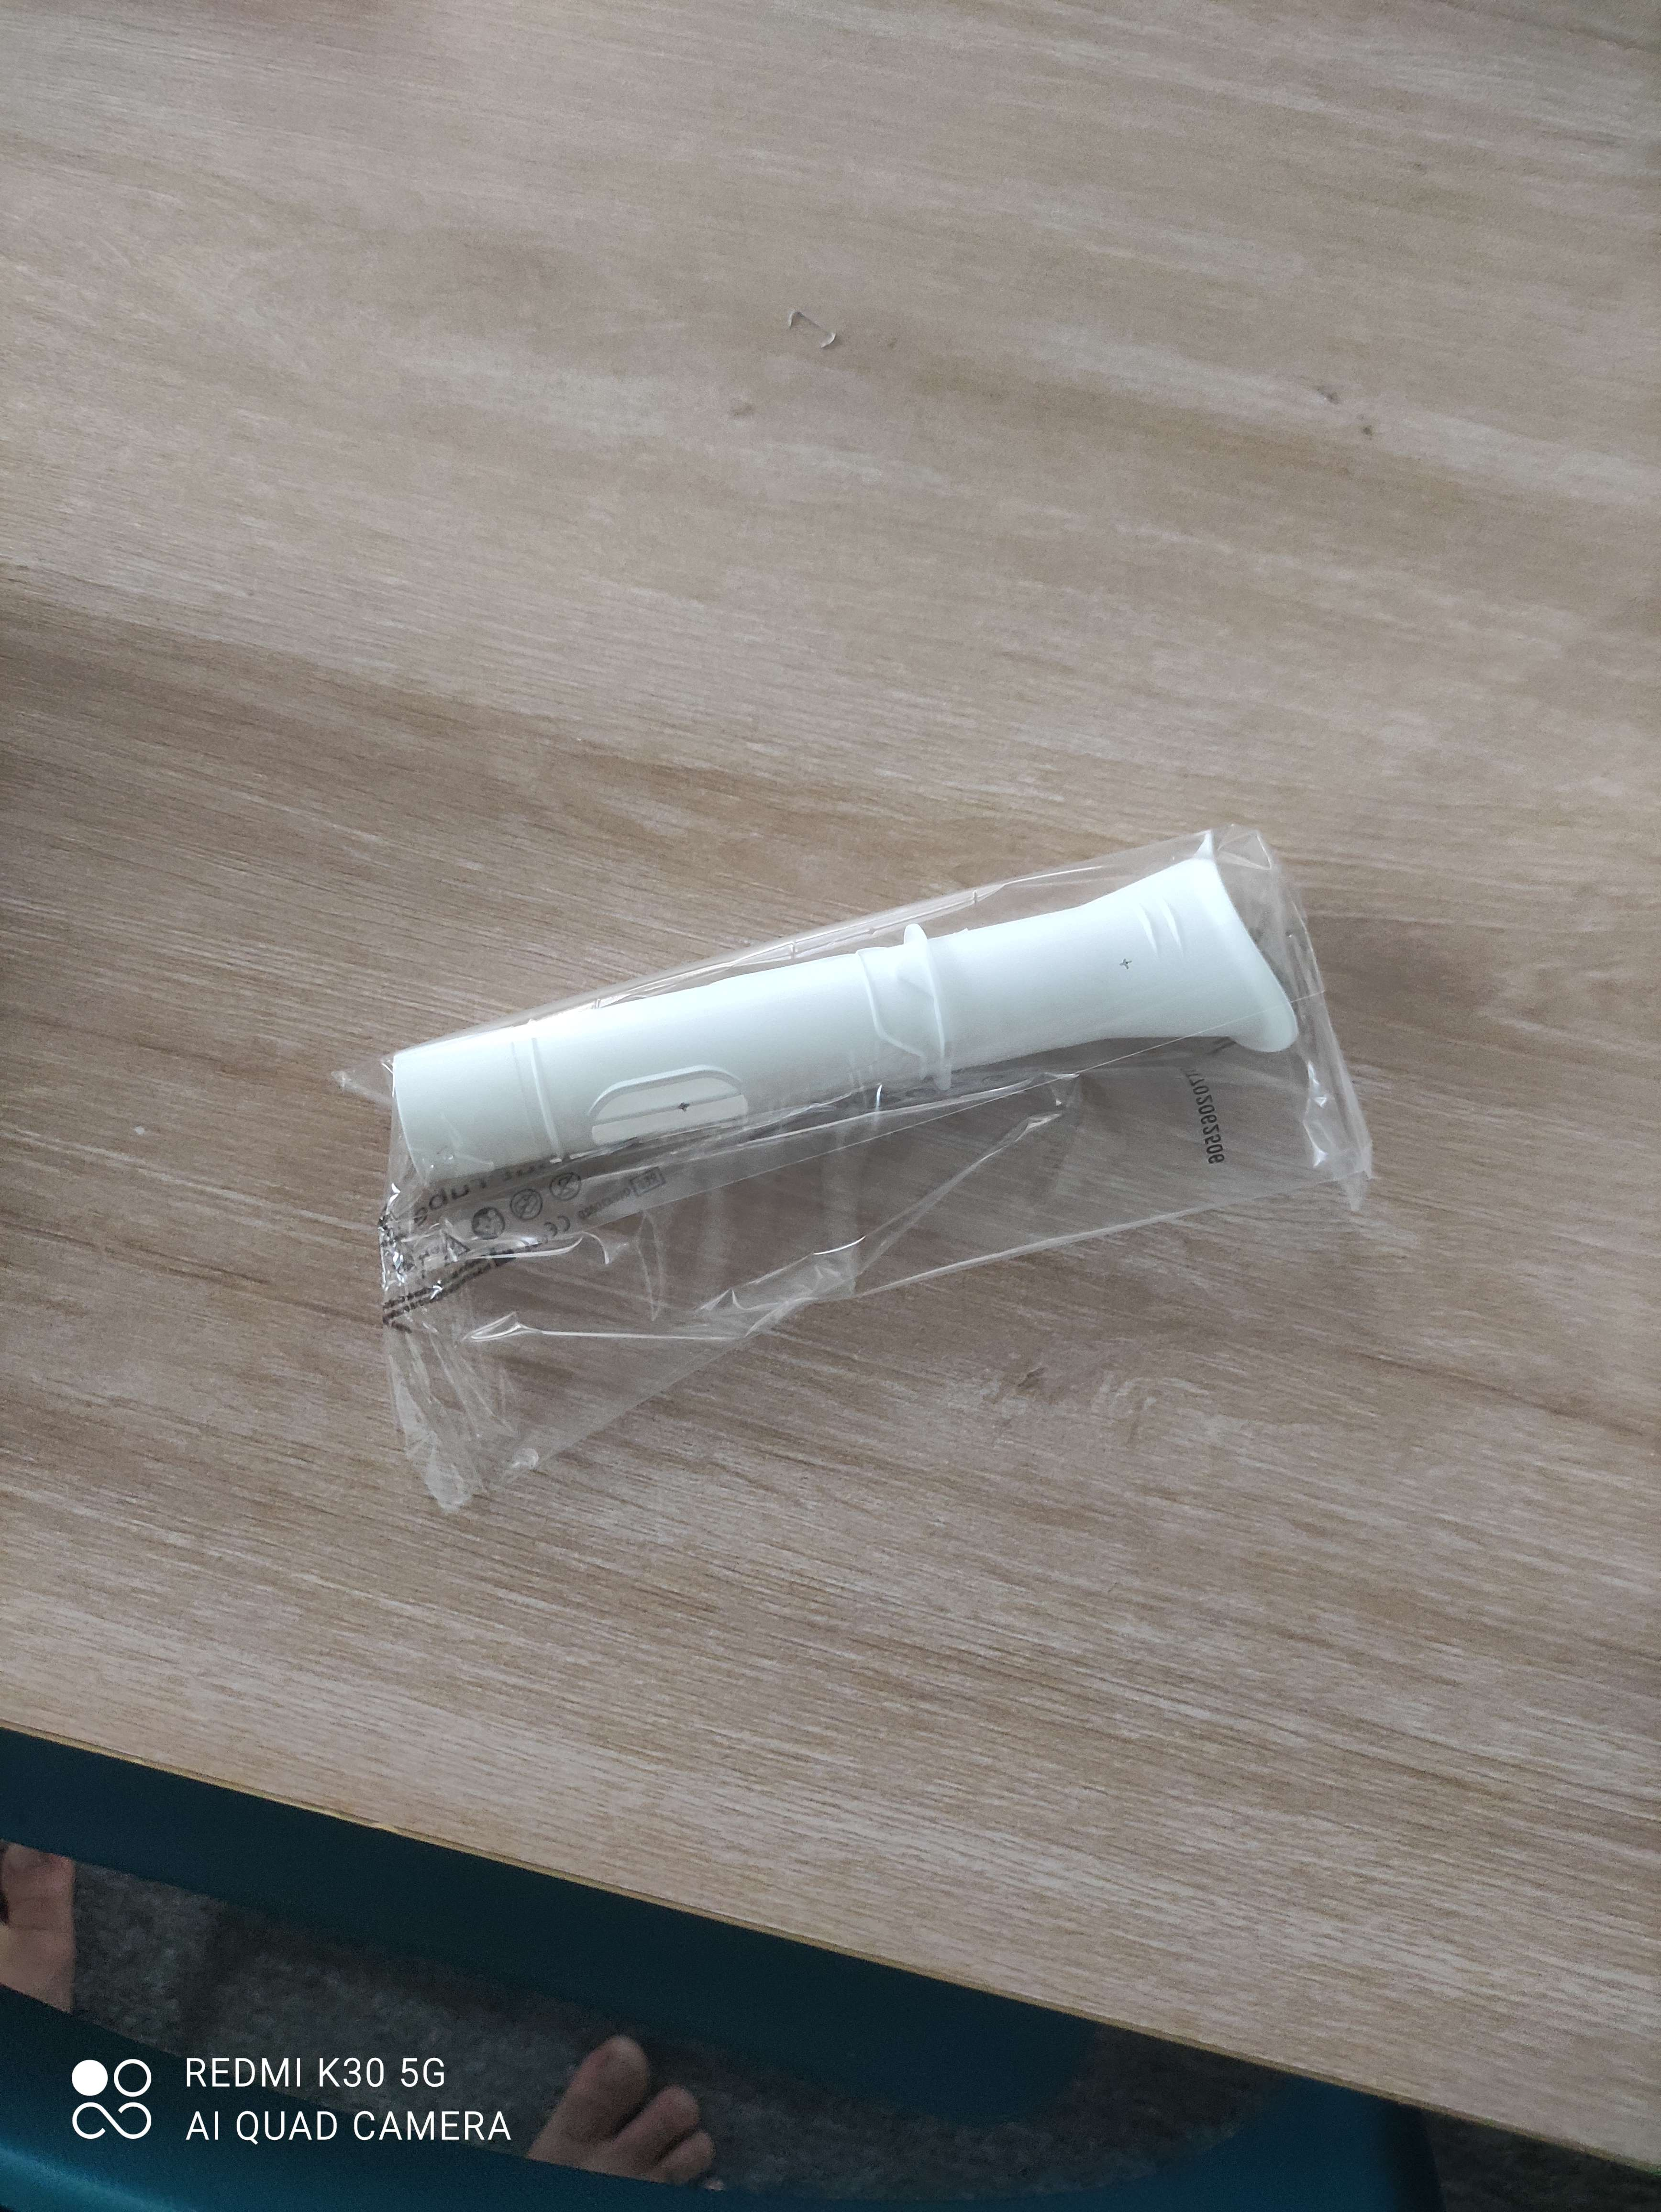
\includegraphics[width=0.5\linewidth]{Real-ScoutTube.png}
    \caption{Hình ảnh thực tế ống lọc PFT}
    \label{fig:placeholder}
\end{figure}

\begin{tabular}{ll}
\toprule
    Thông số kỹ thuật của FPT Filter:\\
    \midrule
   Nhà máy sản xuất  & GANSHORN PTF Filter \\
   \addlinespace
   Loại  & Electrostatic filter, fleece with protective membrane.\\
   \addlinespace
   Bảo vệ vi khuẩn / virus & 99.9999 \% hiệu quả lọc vi khuẩn/virus\\
   \addlinespace
   Sự thoải mái của bệnh nhân & Ống ngậm có hình dáng tiện dụng và hình nón tiêu chuẩn 22 mm \\
   \addlinespace
   Chất liệu & Polypropylen trắng\\
   \addlinespace
   Trở kháng & @ 12 L/s 0.7 cmH20/L/s (0.07 kPa/L/s)\\
   \addlinespace
   Khoang khí chết hiệu dụng & 50 ml\\
   \addlinespace
        & Bộ lọc PFT đáp ứng đầy đủ các khuyến nghị mới nhất từ cả Hiệp hội Hô hấp lồng ngực Hoa Kỳ và Châu Âu (ATS \& ERS)\\
        \addlinespace
    \bottomrule
\end{tabular}

\subsection{Đầu nối, bộ điều khiển và chỉ báo SpiroScout}

\begin{figure}[H]
    \centering
    \includegraphics[width=0.5\linewidth]{SpiroScout-anh2.png}
    \caption{Mặt trước SpiroScout}
    \label{fig:placeholder}
\end{figure}
\begin{figure}[H]
    \centering
    \includegraphics[width=0.5\linewidth]{SpiroScout-anh3.png}
    \caption{Mặt sau SpiroScout}
    \label{fig:placeholder}
\end{figure}

\section{Phần mềm LFX}

Như đã nói ở trên, phần mềm LFX (Lung Function Xperience) là nền tảng phần mềm chuyên dụng được phát triển bởi hãng Garnshorn, hoạt động trên hệ điều hành Windows để điều khiển và vận hành thiết bị SpiroScout. Phần mềm đóng vai trò trung tâm trong việc thu thập tín hiệu thời gian thực từ đầu đo siêu âm, xử lý dữ liệu thô và chuyển đổi thành các biểu đồ, chỉ số lâm sàng có ý nghĩa.\\
\\Với giao diện đồ họa trực quan và hiện đại, LFX được thiết kế để tối ưu hóa quy trình làm việc tại phòng khám, giúp kỹ thuật viên dễ dàng thao tác từ khâu nhập liệu bệnh nhân đến khi xuất báo cáo kết quả.

\begin{figure}[H]
	\centering
	\includegraphics[width=0.5\linewidth]{screen_LFX.png}
	\caption{Màn hình khởi động chương trình LFX}
	\label{fig:screenLFX}
\end{figure}
\subsection{Nhập dữ liệu}

\begin{figure}[H]
	\centering
	\includegraphics[width=0.5\linewidth]{Nhapdulieu.png}
	\caption{Màn hình nhập dữ liệu bệnh nhân}
	\label{fig:placeholder}
\end{figure}
Để đo được kết quả chính xác, người sử dụng cần nhập chính xác các thông tin sau của bệnh nhân: Ngày tháng năm sinh, chiều cao, cân nặng của bệnh nhân, giới tính và cuối cùng là dân tộc. Phần mềm sẽ dựa trên các thông số trên để tính toán các giá trị dưới đây.

\subsection*{Giá trị tính toán của bệnh nhân}
\begin{table}[H]
	\centering
	\small % Dùng font nhỏ hơn một chút để bảng thoáng hơn
	\renewcommand{\arraystretch}{1.5} % Tăng khoảng cách giữa các dòng
	% Cấu trúc: Cột 1 (3cm), Cột 2 (4cm), Cột 3 (Tự động dãn hết phần còn lại)
	\begin{tabularx}{\textwidth}{|p{3cm}|p{4cm}|X|}
		\hline
		\textbf{Giá trị tính toán} & \textbf{Giải thích} & \textbf{Công thức} \\
		\hline
		
		BSA & Diện tích bề mặt cơ thể tính bằng $m^2$ theo Mosteller & 
		\begin{itemize}[nosep, leftmargin=1em, label=\textbullet, before=\vspace*{-\baselineskip}, after=\vspace*{-\baselineskip}]
			\item Công thức dành cho nam và nữ:
			
			\item $BSA = \sqrt{\frac{\text{Chiều cao (cm)} \times \text{Cân nặng (kg)}}{3600}}$
		\end{itemize} \\
		\hline
		
		
		BMI & Chỉ số khối cơ thể tính bằng $kg/m^2$ theo Adolphe Quetelet & 
		\begin{itemize}[nosep, leftmargin=1em, label=\textbullet, before=\vspace*{-\baselineskip}, after=\vspace*{-\baselineskip}]
			\item Công thức dành cho nam và nữ:
			\item $BMI = \frac{\text{Cân nặng (kg)}}{\text{Chiều cao}^2 (m)}$
		\end{itemize} \\
		\hline
		
		Cân nặng lý tưởng (Ideal weight) & Cân nặng lý tưởng tính bằng kg theo Dr. Devine & 
		\begin{itemize}[nosep, leftmargin=1em, label=\textbullet, before=\vspace*{-\baselineskip}, after=\vspace*{-\baselineskip}]
			\item \textbf{Nam:} $50 + 2,3$ kg cho mỗi inch trên 5 feet.
			\item \textbf{Nữ:} $45,5 + 2,3$ kg cho mỗi inch trên 5 feet.
		\end{itemize} \\
		\hline
		
		Trọng lượng tương đối (Rel. weight) & Trọng lượng tương đối tính bằng \% & 
		\begin{itemize}[nosep, leftmargin=1em, label=\textbullet, before=\vspace*{-\baselineskip}, after=\vspace*{-\baselineskip}]
			\item Công thức dành cho nam và nữ:
			\item $\text{TL tương đối} = \frac{\text{Cân nặng (kg)}}{\text{Chiều cao (cm)} - 100} \times 100$
		\end{itemize} \\
		\hline
		
		LBW & Trọng lượng cơ thể nạc tính bằng kg theo James & 
		\tabitem \textbf{Nam:} $LBW = (1.10 \times \text{Cân nặng}) - 128 \times (\frac{\text{Cân nặng}}{100 \times \text{Chiều cao}})^2$ \newline
		\tabitem \textbf{Nữ:} $LBW = (1.07 \times \text{Cân nặng}) - 148 \times (\frac{\text{Cân nặng}}{100 \times \text{Chiều cao}})^2$ \\
		\hline
		
		Chiều cao từ khoảng cách cánh tay & Công thức dùng ước tính chiều cao bệnh nhân & 
		\tabitem \textbf{Tuổi < 18 (Hibbert, Torres):} \newline 
		$\text{Chiều cao (cm)} = \text{Sải tay (cm)}$ \newline
		\tabitem \textbf{Tuổi > 18 (Parker và cộng sự):} \newline
		$\text{Chiều cao} = 67,90 + 0,664182 \times \text{Sải tay} + 2,816 \times \text{Giới tính} - 4,05 \times \text{Chủng tộc} - 0,0709 \times \text{Tuổi}$ \newline
		\textit{(Trong đó: Giới tính: 1=Nam, 2=Nữ; Chủng tộc: 1=Trắng, 2=Đen)} \\
		\hline
		
		Pack years (Hút thuốc) & Công thức tính số năm hút thuốc & 
		\tabitem $\text{Năm} = \frac{\text{Thuốc lá mỗi ngày}}{\text{Thuốc lá mỗi gói}} \times \text{Số năm hút thuốc}$ \\
		\hline
	\end{tabularx}
\end{table}

\section{Nguyên lý đo lường}
Máy SpiroCount sử dụng công nghệ đo lưu lượng bằng cảm biến siêu âm (Ultrasonic Flow Measurement) thay vì sử dụng tuabin quay hay cảm biến chênh áp truyền thống. Nguyên lý hoạt động dựa trên sự thay đổi thời gian truyền của sóng âm khi đi qua dòng khí đang chuyển động.
\section*{Cấu tạo cảm biến}
Hệ thống đo lượng bao gồm một ống thở và hai đầu dò siêu âm được bố trí đối diện nhau theo một đường chéo cắt ngang dòng khí.
\begin{figure}[H]
    \centering
    \includegraphics[width=0.5\linewidth]{measurement-principle.png}
    \caption{Cảm biến lưu lượng siêu ẩm}
    \label{fig:placeholder}
\end{figure}

\section*{Quy trình đo lường}
Quá trình xác định lưu lượng khí thở diễn ra theo các bước sau:
\begin{enumerate}
	\item \textbf{Phát -- Thu tín hiệu:} Hai đầu dò siêu âm hoạt động luân phiên, vừa là bộ phát vừa là bộ thu. Chúng liên tục gửi các xung sóng siêu âm qua lại cho nhau: một xung đi xuôi theo chiều dòng khí và một xung đi ngược chiều dòng khí.
	
	\item \textbf{So sánh thời gian truyền (Transit-time):}
	\begin{itemize}
		\item \textbf{Khi không có dòng khí (Lưu lượng = 0):} Thời gian truyền sóng của hai hướng là bằng nhau.
		\item \textbf{Khi bệnh nhân thở (Có dòng khí):} Dòng khí sẽ làm tăng tốc độ sóng âm đi "xuôi dòng" và làm chậm tốc độ sóng âm đi "ngược dòng".
	\end{itemize}
	
	\item \textbf{Tính toán kết quả:}
	\begin{itemize}
		\item Máy sẽ đo sự chênh lệch thời gian ($\Delta t$) giữa hai xung sóng. Sự chênh lệch này tỷ lệ thuận trực tiếp với vận tốc của dòng khí.
		\item Từ vận tốc dòng khí và tiết diện ống thở, bộ vi xử lý sẽ tính toán ra \textbf{Lưu lượng (Flow)} và \textbf{Thể tích (Volume)} khí thở của bệnh nhân.
	\end{itemize}
\end{enumerate}


\section{Quy trình vận hành}
\subsection{Quá trình lắp đặt và chuẩn bị ban đầu}
\begin{enumerate}
	\item{Kết nối SpiroCount với PC}
	\begin{enumerate}
		\item Đảm bảo PC đã tắt.
		\item Tại SpiroScout, kết nối cáp cảm biến giữa đầu nối RS232 trên Cảm biến và đầu nối RS232 trên đế.
		\item Sử dụng cáp USB để truyền dữ liệu với PC. Đầu nối cổng USB ở trạm gốc với cổng USB miễn phí trên PC.
		\item Nếu hệ thống của bạn được cung cấp bộ chuyển đổi AC riêng, hãy kết nối bộ chuyển đổi AC với ổ cắm DC-IN.
	\end{enumerate}
	
	\item{Khởi động hệ thống}
	\begin{enumerate}
		\item Bật PC
		\item Bật SpiroScout bằng công tắc nguồn ở phía sau trạm gốc.\\ Kiểm tra xem đèn báo nguồn ở mặt trước của bộ phận đế có sáng đỏ hay không.Tín hiệu được đưa ra khi bật lần đầu tiên. Điều này cho thấy SpiroScout đã sẵn sàng để sử dụng.
		\item Khởi động chương trình LFX từ màn hình nền Windows bằng cách nhấp đúp vào biểu tượng LFX.
	\end{enumerate}
\end{enumerate}
\subsection{Lắp bộ lọc thở PFT dùng một lần}
\begin{enumerate}
	\item Dụng cụ thở dùng một lần
	\begin{itemize}
		\item Ống thở SpiroScout (SpiretteTM) là vật dụng dùng một lần và không được tái sử dụng. Một cái mới phải được sử dụng cho mỗi bệnh nhân. Không sử dụng cho nhiều hơn một bệnh nhân.
		\item Không cố gắng làm sạch
	\end{itemize}
	\begin{figure}[H]
		\centering
		\includegraphics[width=0.5\linewidth]{setting-PFT-filter.png}
		\caption{Lắp đặt ống thở lọc khuẩn PFT}
		\label{fig:placeholder}
	\end{figure}
	\item Tháo miếng đệm thở
	Để tháo miếng đệm thở, hãy kéo nó ra khỏi giá đỡ ScoutSensor, xoay nó ngược chiều kim đồng hồ một chút nếu cần.
	\item Lắp bộ lọc vi khuẩn PFT
	\begin{itemize}
		\item Chỉ sử dụng một lần - không sử dụng bộ lọc PFT cho nhiều bệnh nhân.
		\item Không cố gắng làm sạch bộ lọc.
		\item Chỉ sử dụng bộ lọc vi khuẩn được GANSHORN phê duyệt. Việc sử dụng bất kỳ bộ lọc nào khác có thể gây ra kết quả đo không chính xác.
	\end{itemize}
	Bộ lọc vi khuẩn là bộ lọc vi khuẩn sử dụng một lần được thiết kế để giúp giảm thiểu nguy cơ ô nhiễm không khí và nguy cơ lây nhiễm chéo khi thực hiện các xét nghiệm chức năng phổi và vừa khít với ống ngậm để tạo thành một miệng bịt kín khí.\\
\end{enumerate}
\section*{Kiểm tra trong suốt quá trình lắp đặt}
\begin{itemize}
	\item Quan sát tất cả các quy trình lây nhiễm chéo, ví dụ: đeo găng tay cao su, không để chất thải y tế tiếp xúc với bất kỳ ai, loại bỏ và vứt bỏ màng lọc vi khuẩn vào trong chất thải y tế.
	\item Lau/làm sạch ScoutSensor bằng dung dịch làm sạch hoặc chất khử trùng đã được phê duyệt
\end{itemize}
\subsection{Làm sạch và khử trùng}
SpiroScout và bộ phận đế có thể được lau bằng vải ẩm để làm sạch. Có thể sử dụng chất khử trùng tiêu chuẩn của bệnh viện để khử trùng SpiroScout.
Cảm biến siêu âm phải được khử trùng hằng tuần.

\subsection{Xác minh và hiệu chỉnh}
SpiroScout kết hợp các cảm biến áp suất và độ ẩm,  và vì SpiroScout hoạt động dựa trên việc đo thời gian truyền sóng âm nên việc hiệu chuẩn thể tích hằng ngày là hoàn toàn không cần thiết. Hiện tại thiết bị chỉ cần hiệu chỉnh điểm 0, một số tham số phụ của môi trường bên ngoài, và thể tích theo yêu cầu của tiêu chuẩn quốc tế 
\subsubsection{Hiệu chuẩn điểm 0}
Hiệu chuẩn điểm 0 được thực hiện tự động khi bật nguồn và sau 15 phút mỗi lần. Trong quá trình điều chỉnh về 0, máy xác định trạng thái "tĩnh" của dòng khí trong ống đo để thiết lập mức tham chiếu. Lưu ý:
\begin{itemize}
	\item Không di chuyển cảm biến.
	\item Không thở vào cảm biến.
	\item Ngăn gió lùa vào, đóng cửa sổ phòng, và không di chuyển bất kỳ bộ phận nào của thiết bị.
\end{itemize}
\subsubsection{Thông số môi trường xung quanh}
Dựa trên các giá trị được hệ thống đo trực tiếp, nhiệt độ $[^\circ C]$ và áp suất xung quanh $[hPa]$, cũng như các giá trị được cài đặt thủ công, độ ẩm $[\%]$ và độ cao so với mực nước biển $[m]$, các thông số môi trường này cần được cập nhập theo định kỳ để đảm bảo phép đo chính xác nhất, chương trình LFX xác định hệ số điều chỉnh thể tích STPD và BTPS.\\
Trong đó:
\begin{itemize}
	\item BTPS (Body Temperature, Pressure, Saturated): 
	Đây là điều kiện khí bên trong cơ thể (phổi) của con người. 
	\begin{itemize}
		\item Body Temperature: Nhiệt độ cơ thể, thường lấy ở $37^\circ C$ hay 310K.
		\item Pressure: Áp suất khí quyển tại nơi đo.
		\item Saturated: Bão hoà hơi nước (độ ẩm $100\%$ tại $37^\circ C$, áp suất hơi nước khoảng 47 mmHg).
	\end{itemize}
	\item STPD (Standard Temperature, Pressue, Dry): Điều kiện khí tiêu chuẩn, thường dùng trong các nghiệm pháp gắng sức tim mạch - hô hấp, để đo sự tiêu thụ $O_2$ hoặc thải $CO_2$.
\end{itemize}
\subsubsection{Hiệu chuẩn thể tích}
Để đảm bảo độ tin cậy cho hệ thống, và tuân thủ các tiêu chuẩn quốc tế, thể tích có thể được hiệu chuẩn theo các yêu cầu dưới đây:
\begin{itemize}
	\item Chỉ sử dụng ống tiêm hiệu chuẩn ban đầu và bộ chuyển đổi silicon do GANSHORN cung cấp hoặc phê duyệt. Ống tiêm hiệu chuẩn phải được xác minh thường xuyên.
	\item Việc xác minh và hiệu chuẩn thể tích được thực hiện bằng ống tiêm hiệu chuẩn được kết nối với cảm biến và xả/sạc ở tốc độ ổn định với phạm vi lưu lượng trong khoảng từ 0.5 đến 1.2 lít trên giây.
	\item Kết quả đo được phải nằm trong sai số $\pm 3.5\%$ (bao gồm cả độ chính xác $0.5\%$ của ống tiêm). 
\end{itemize}
\subsubsection{Quy trình hiệu chuẩn thể tích}
\begin{enumerate}
	\item Lắp ống thở mới hoặc đặt bộ lọc vi khuẩn PFT mới vào cảm biến.
	\item Từ màn hình bệnh nhân, nhấp vào nút Calib.
	\item Cài đặt hiệu chỉnh được hiển thị ở bên phải màn hình.
	\item Nhấp vào Vol để vào màn hình hiểu chuẩn.
	\item Nhập thể tích của ống tiêm hiệu chuẩn (Nên dùng ống tiêm 3 lít).
	\item Kết nối ống tiêm hiệu chuẩn với bộ chuyển đổi silicon và bộ lọc PFT.
	\item Đảm bảo tiếp xúc tốt và không rò rỉ.
	\item Nhấp vào nút bắt đầu.\\
	Một thông báo hiện ra: \textit{Calibrating Offset. Please don’t breathe or create any flow in front of the sensor}
	\item Sau một lúc, độ lệch được hiệu chỉnh và màn hình hiển thị thể tích hiện lên. Kéo piston nhẹ nhàng qua lại với lưu lượng không đổi từ 0.5 đến 12 L/s.
	\item Sau vài lần bơm, chương trình sẽ tự động dừng và hiện thị thông báo thành công hoặc thất bại.
\end{enumerate}
\begin{figure}[H]
	\centering
	\includegraphics[width=0.5\linewidth]{volume_calibration.png}
	\caption{Màn hình hiệu chuẩn thể tích}
	\label{fig:volume_calibration}
\end{figure}
\subsubsection{Kết quả dạng bảng sau khi hiệu chuẩn}
Thể tích sau khi hiệu chuẩn sẽ được hiển thị trong kết quả dạng bảng. Thể tích ở mỗi luồng phải đáp ứng yêu cầu về độ chính xác là $3.5\%$ (bao gồm độ chính xác $0.5\%$ của ống tiêm). Đối với ống tiêm 3 lít, thể tích đo được ở mỗi lần bơm phải nằm trong khoảng 2.895 và 3.105 lít.\\
Chúng ta có thể tăng tốc độ dòng từ 0.5 L/s lên 6L/s rồi 12L/s để kiểm tra độ tuyến tính của cảm biến lưu lượng.
\subsection{Kết quả tốt nhất và giá trị dự đoán}
Theo tiêu chuẩn đo phế dung của Hiệp hội Lồng ngực Hoa Kỳ (ATS) (ngày 11 tháng 11 năm 1994), phép đo tốt nhất được xác định là giá trị cao nhất từ phép tính:
$$\text{Best} = \text{FVC} + \text{FEV1(or FEV6)}$$
Chương trình đo phế dung lấy giá trị tốt nhất được xác định ở trên và xác định giá trị này là 'lựa chọn ưu tiên'  theo khuyến nghị của ATS và ERS.
\subsection{Tổng quan phép đo}
\subsubsection{Đo phế dung chậm}
Đo phế dung chậm được thực hiện để đo thể tích phổi hít vào và thở ra (SVC, VCin, VCex, ERV, IC, v.v.v.) trong các thao tác chậm. Nó đo lượng không khí một người hít vào và thở ra theo thời gian.\\
Nên thực hiện các thao tác VC trước các thao tác FVC vì có khả năng xảy ra tắc nghẽn phế quản hoặc giãn phế quản sau khi thực hiện các thao tác cưỡng bức.\\
Trong quá trình thực hiện thủ thuật này, bệnh nhân nên thở bình thường 3 lần rồi hít vào càng nhiều càng tốt cho dung tích phổi tối đa, sau đó thở ra hết sức có thể.
\subsubsection*{Thông số đo}
Dung tích sống (VC) có thể đo được bằng cách thực hiện thao tác thở theo 2 cách khác nhau. 

\begin{enumerate}
	\item \textbf{Động tác hít vào gắng sức(IVC maneuverer)}\\
	Sau một thời gian thở nhẹ và đều đặn (thở bình thường), bệnh nhân thở ra hoàn toàn, sau đó hít vào hoàn toàn. IVC(Inspiratory Vital Capacity) là dung tích hít vào, đây là lượng khí tối đa mà một người có thể hít vào sau khi đã thở ra hết sức.
	\begin{figure}[H]
		\centering
		\includegraphics[width=0.5\linewidth]{IVC.png}
		\caption{Giản đồ ghi lại thể tích phổi theo thời gian trong IVC}
		\label{fig:IVC}
	\end{figure}
	\item \textbf{Động tác thở ra gắng sức (EVC maneuverer)}\\
	Sau một thời gian thở nhẹ và đều đặn, bệnh nhân hít vào hoàn toàn, sau đó thở ra hoàn toàn. EVC(Expiratory Vital Capacity) là dung tích khí mà một người có thể thở ra sau khi hít vào hết sức, với tốc độ thở từ từ, không gấp gáp.
	\begin{figure}[H]
		\centering
		\includegraphics[width=0.5\linewidth]{EVC.png}
		\caption{Giản đồ ghi lại thể tích phổi theo thời gian trong EVC}
		\label{fig:EVC}
	\end{figure}
\end{enumerate}
\subsubsection*{Các thông số khác được đo trong quá trình đo Phế dung ký chậm}
\begin{itemize}
	\item BF = Breathing Frequency (1/min) : Số nhịp thở bệnh nhân thực hiện trong một phút.
	\item MV = Minute Volume (L/min) : Là tổng lượng khí được hít vào hoặc thở ra trong một phút. = BF * VT(Thể tích khí lưu thông)
	\item VC MAX = Maximal Vital Capacity (L) : Là giá trị dung tích sống cao nhất ghi nhận được. Máy sẽ tự động so sánh và chọn giá trị lớn hơn giữa $VC_{IN}$ (Dung tích sống hít vào) hoặc $VC_{EX}$ (Dung tích sống thở ra).
	\item T EX = Time expiatory tidal breath (sec). : Thời gian của thì thở ra trong một nhịp thở thường.
	\item T IN = Time inspiratory tidal breath (sec).: Thời gian của thì hít vào trong một nhịp thở thường.
	\item T TOT = Time complete tidal breathing manouvre (sec).: Tổng thời gian để hoàn thành trọn vẹn một chu kỳ thở thường (bao gồm hít vào và thở ra).
	\item TI/TE = Ratio of the T IN and T EX: Tỷ lệ giữa thời gian hít vào ($T_{IN}$) và thời gian thở ra ($T_{EX}$).
\end{itemize}
\subsubsection{Đo phế dung cưỡng bức}
Phép đo phế dung cưỡng bức được thực hiện để đo thể tích và lưu lượng thở ra và hít vào trong quá trình gắng sức tối đa. Nó đo lường cách một người hít vào thở ra mạnh một lượng không khí. Các phép đo chính như sau :
\begin{enumerate}
	\item \textbf{Dung tích sống gắng sức - Forced Vital Capacity (FVC)}: Lượng khí (tính bằng lít) đo được trong quá trình thở ra mạnh và hết sức có thể, bắt đầu từ vị trí hít vào đầy phổi.
	\item \textbf{Thể tích thở ra gắng sức trong giây đầu - The forced expiratory volume in one second (FEV1)}: Lượng khí (tính bằng lít) đo được trong giây đầu tiên của nghiệm pháp thở ra gắng sức.
\end{enumerate}
\subsubsection*{Thông số đo}
Trong quá trình đo phế dung cưỡng bức, chúng ta đo các thông số liên quan đến thể tích và lưu lượng trong các thao tác cưỡng bức.
\begin{enumerate}
	\item \textbf{Các thông số thể tích}: Dung tích sống gắng sức (FVC) và thể tích thở ra gắng sức trong 1s (FEV1) đều được biểu thị bằng lít. Ngoài 2 thông số này, chúng ta còn có thể đo: IRV, VT, ERV và IC. 
	\begin{figure}[H]
		\centering
		\includegraphics[width=0.8\linewidth]{volume.png}
		\caption{Volume related parameters}
		\label{fig:volume}
	\end{figure}
	\item \textbf{Các thông số lưu lượng}: Lưu lượng thở ra tối đa được xác định từ thở ra gắng sức tối đa được gọi là lưu lượng thở ra cao nhất (PEF). Lưu lượng hít vào tối đa (PIF) và lưu lượng hít vào tối đa được xác định từ hít vào tối đa. Ngoài ra, chúng ta cũng có thể đo lưu lượng thở ra ở một thể tích dài cụ thể trong thao tác thở ra gắng sức (VD: MEF75, MEF50, MEF25).
	\begin{figure}[H]
		\centering
		\includegraphics[width=0.8\linewidth]{flow.png}
		\caption{Flow related parameters}
		\label{fig:flow}
	\end{figure}
\end{enumerate}
\subsubsection*{Các thông số khác được đo trong quá trình đo Phế dung cưỡng bức}
\begin{itemize}
	\item FVC IN = Dung tích sống hít vào cưỡng bức(L)
	\item FIV1 = Dung tích hít vào cưỡng bức trong 1s (L)
	\item FIV0.5 = Dung tích hít vào cưỡng bức trong 0.5s (L)
	\item FIV.75 = Dung tích hít vào cưỡng bức trong 0.75s (L)
	\item FIV2 = Dung tích hít vào cưỡng bức trong 2s (L)
	\item FIV3 = Dung tích hít vào cưỡng bức trong 3s (L)
	\item FIV6 = Dung tích hít vào cưỡng bức trong 6s (L)
	\item MMEF = Lưu lượng thở ra tối đa giữa thì (L/s)
	\item VC IN = Dung tích sống hít vào (L)
	\item VC EX = Dung tích sống thở ra (L)
	\item VC MAX = Dung tích sống đo được tối đa (L)
	\item EV = Dung tích thở ra (L)
	\item $\text{EV\%FVC}$ = Dung tích thở ra theo phần trăm của FCV($ \% $).
	\item PEFT = Thời gian cho đến khi đạt lưu lượng thở ra cao nhất (sec).
	\item AEX = Diện tích đường cong thở ra ($L*L/s $)
	\item AIN = Diện tích đường cong hít vào ($L*L/s $)
	\item BF = Tần suất thở (1/min)
	\item MV = Thông khí tối đa (L/min)
	\item T EX =  Thời gian của thì thở ra trong một nhịp thở thường (sec).
	\item T IN = Thời gian của thì hít vào trong một nhịp thở thường.
	\item T TOT =Tổng thời gian để hoàn thành trọn vẹn một chu kỳ thở thường (bao gồm hít vào và thở ra).
	\item TI/TE =Tỷ lệ giữa thời gian hít vào ($T_{IN}$) và thời gian thở ra ($T_{EX}$).
\end{itemize}

\subsubsection{Kiểm soát chất lượng trong quá trình đo}
Tiêu chí kết thúc thử nghiệm đạt được khi: thời gian thở ra là $\ge$ 6 giây (3 giây ở trẻ > 10 tuổi) hoặc khi thể tích < 25 ml trong một giây.
Theo hướng dẫn ATS/ERS 2005, tiêu chí cuối cùng của bài kiểm tra được đáp ứng khi ít nhất đạt được một trong 2 tiêu chí này.
\section{Hình ảnh của một số phép đo}
\subsection{Đo phế dung ký chậm}
\begin{figure}[H]
	\centering
	\includegraphics[width=0.8\linewidth]{SV_review.png}
	\caption{Đang thực hiện đo phế dung ký chậm}
\end{figure}

\begin{figure}[h]
	\centering
	% ---------------- HÀNG 1: HÌNH TRÊN ----------------
	% Cột bên trái: Chứa Caption 1
	\begin{minipage}[c]{0.35\textwidth} 
		\caption{Biểu đồ minh họa quá trình hít vào (IVC). Đường cong đi lên thể hiện dung tích hít vào tối đa.}
		\label{fig:hinh_tren}
	\end{minipage}
	\hfill % Đẩy hình sang phải
	% Cột bên phải: Chứa Hình 1
	\begin{minipage}[c]{0.6\textwidth}
		\centering
		\includegraphics[width=\linewidth]{IVC_review.png} 
	\end{minipage}
	
	% Tạo khoảng cách giữa 2 hình (quan trọng)
	\vspace{1cm} 
	
	% ---------------- HÀNG 2: HÌNH DƯỚI ----------------
	% Cột bên trái: Chứa Caption 2
	\begin{minipage}[c]{0.35\textwidth} 
		\caption{Biểu đồ minh họa quá trình thở ra (EVC). Đường cong đi xuống thể hiện dung tích thở ra tối đa.}
		\label{fig:hinh_duoi}
	\end{minipage}
	\hfill % Đẩy hình sang phải
	% Cột bên phải: Chứa Hình 2
	\begin{minipage}[c]{0.6\textwidth}
		\centering
		\includegraphics[width=\linewidth]{EVC_review.png} 
	\end{minipage}
\end{figure}

\begin{figure}[H]
	\centering
	\includegraphics[width=0.8\linewidth]{SVC_review.png}
	\caption{Kết quả cuối cùng của đo phế dung ký chậm}
\end{figure}
\textbf{Nhận xét}: SVC dùng để xác nhận xem phổi có bị nhỏ đi hay cứng lại không (như trong bệnh xơ phổi, vẹo cột sống, béo phì).
\subsection{Đo phế dung ký cưỡng bức}

\begin{figure}[H]
	\centering
	\includegraphics[width=0.8\linewidth]{Forced_review.png}
	\caption{Kết quả cuối cùng của đo phế dung ký cưỡng bức}
\end{figure}
\textbf{Nhận xét}: Đo xem bệnh nhân có thể thổi ra mạnh, nhanh và nhiều đến mức nào. Đây là nghiệm pháp quan trọng nhất để chẩn đoán tắc nghẽn đường thở (như trong bệnh COPD hoặc Hen suyễn).
\section{Xử lý sự cố}
\begin{longtable}{|p{3.5cm}|p{5cm}|p{6cm}|}
	\hline
	\textbf{Thông báo lỗi } & \textbf{Kiểm tra / Quy trình / Nguyên nhân có thể} & \textbf{Cách khắc phục } \\ \hline
	% --- Hàng 1 ---
	Không có giao tiếp dữ liệu với cảm biến phế dung (No Data Communication with spiro sensor) & 
	\begin{itemize}[leftmargin=*, nosep]
		\item Hệ thống bị mất cổng giao tiếp với cảm biến.
		\item Thiết bị hoặc cổng được xác định không chính xác.
	\end{itemize} & 
	\begin{itemize}[leftmargin=*, nosep]
		\item Kiểm tra trong cài đặt hệ thống xem thiết bị và cổng chính xác đã được xác định chưa (xem phần 6, Khắc phục sự cố, trang 52).
		\item Trong cài đặt hệ thống, chọn tùy chọn \textbf{Remove device} để gỡ thiết bị. Sau đó chọn \textbf{Add device} với đúng thiết bị / cổng để thực hiện cài đặt mới sạch sẽ.
	\end{itemize} \\ \hline
	
	% --- Hàng 2 ---
	Không thể thực hiện ghi Phế dung ký (Not possible to take a Spiro Recording) & 
	\begin{itemize}[leftmargin=*, nosep]
		\item Bộ lọc khuẩn PFT bị lỗi.
		\item Ống thở dùng một lần bị lỗi.
		\item Đầu dò lưu lượng (Flow transducer) bị lỗi (chỉ khi sử dụng đầu dò vĩnh cửu kết hợp với bộ lọc PFT).
	\end{itemize} & 
	\begin{itemize}[leftmargin=*, nosep]
		\item Thay thế bộ lọc PFT.
		\item Thay thế ống thở.
		\item Tháo và vệ sinh cảm biến dòng chảy (xem phần 8.4.5, Lắp ráp và Tháo gỡ Đầu dò Siêu âm, trang 57).
		\item Thay thế cảm biến dòng chảy.
	\end{itemize} \\ \hline
	
	% --- Hàng 3 ---
	Thông báo lỗi Điểm chuẩn / Đường cơ sở (Zero point / baseline error) & 
	\begin{itemize}[leftmargin=*, nosep]
		\item Việc thiết lập điểm chuẩn (Zero point) được thực hiện tự động khi bật máy LFX và lặp lại mỗi 15 phút trong quá trình sử dụng. Nếu độ lệch quá lớn, thông báo lỗi sẽ hiển thị.
	\end{itemize} & 
	\begin{itemize}[leftmargin=*, nosep]
		\item Đảm bảo thời gian khởi động máy ít nhất 30 phút.
		\item Kiểm tra xem cảm biến có được giữ yên tĩnh trong quá trình zeroing không.
		\item Đảm bảo phòng không có gió lùa và nhiệt độ đồng đều. Đóng các cửa sổ.
		\item Tắt mọi thiết bị điều hòa không khí trong phòng.
		\item Đảm bảo không có hơi thở nào ảnh hưởng đến quá trình zeroing - di chuyển bệnh nhân / người vận hành ra xa cảm biến.
		\item Thay thế bộ lọc khuẩn PFT.
	\end{itemize} \\ \hline
	
\end{longtable}

\section{Bảo trì}
Trước mỗi lần vận hành, cần kiểm tra trực quan thiết bị, dây cáp và đầu nối:

\begin{itemize}
	\item Tìm kiếm dấu hiệu hư hỏng vật lý hoặc suy giảm chức năng.
	\item Kiểm tra dây cáp (uốn nhẹ để xem có bị mòn/hở dây không) và độ chắc chắn của các đầu nối.
	\item \textbf{Lưu ý:} Nếu phát hiện hư hỏng, ngừng sử dụng ngay lập tức và liên hệ bộ phận kỹ thuật.
\end{itemize}
\subsection{Dịch vụ kỹ thuật}
Thiết bị không chứa các bộ phận người dùng có thể tự thay thế. Việc sửa chữa phải được thực hiện bởi đơn vị ủy quyền của nhà sản xuất.

\subsection{Quy trình Vệ sinh và Khử trùng}
\textbf{Cảnh báo:} Không tái sử dụng vật tư tiêu hao (ống thở, lọc khuẩn, kẹp mũi dùng một lần) để tránh lây nhiễm chéo. Luôn đeo găng tay và kính bảo hộ khi vệ sinh.

\subsubsection{Vệ sinh thiết bị và dây cáp}
\begin{itemize}
	\item Lau bằng vải ẩm (không ướt) với dung dịch được phê duyệt.
	\item Không để chất lỏng lọt vào các khe hở hoặc đầu nối.
	\item Tuyệt đối \textbf{KHÔNG} dùng: Cồn etylic, Axeton, Hexan, hoặc chất tẩy rửa có tính axit cao (gây hỏng nhựa).
	\item Không hấp tiệt trùng (Autoclave) hoặc nhúng thiết bị vào nước.
\end{itemize}

\subsubsection{Vệ sinh đầu dò siêu âm (Hàng tuần)}
\begin{enumerate}
	\item Tháo rời các bộ phận (miếng đệm thở, bộ chuyển đổi).
	\item Rửa sạch bằng nước, sau đó ngâm trong dung dịch khử trùng theo quy định.
	\item Rửa lại bằng nước sạch và để khô hoàn toàn trước khi lắp ráp.
	
\end{enumerate}

\subsection{Lắp ráp và tháo dời đầu dò siêu âm}
\subsubsection{Tháo miếng đệm thở}
Để tháo miếng đệm thở cố định, hãy tháo đai ốc đếm và rút miếng đệm ra, xoay nó ngược chiều kim đồng hồ một chút nếu cần.
\begin{figure}[H]
	\centering
	\includegraphics[width=0.5\linewidth]{craft1.png}
\end{figure}
\subsubsection{Thay miếng đệm thở}
\begin{enumerate}
	\item Vặn bộ chuyển đổi màn trập thích hợp vào miếng đệm thở cố định.
	\begin{figure}[H]
		\centering
		\includegraphics[width=0.3\linewidth]{craft2.png}
	\end{figure}
	\item Đưa miếng đệm thở vào ScoutSensor bằng mọi cách.
	\item Căn chỉnh mũi tên trên miếng đệm thở cố định với rãnh trên ScoutSensor và siết chặt miếng đệm thở cố định trong ScoutSensor bằng đai ốc dếm.
	\begin{figure}[H]
		\centering
		\includegraphics[width=0.5\linewidth]{craft3.png}
	\end{figure}
	
\end{enumerate}
\subsubsection{Bộ phận lắp ráp ống thở có thể tái sử dụng}
Phần chèn có thể tái sử dụng bao gồm 4 phần.
	\begin{figure}[H]
	\centering
	\includegraphics[width=0.7\linewidth]{craft4.png}
\end{figure}
\begin{enumerate}
	\item Đưa miếng kim loại vào giá đỡ bằng nhựa. Đảm bảo đường ống của nối kim loại không thẳng hàng với các phần hở trong giá đỡ nhựa.
	\begin{figure}[H]
		\centering
		\includegraphics[width=0.5\linewidth]{craft5.png}
	\end{figure}
	\item Vặn bộ chuyển đổi vào giá đỡ nhựa.
	\begin{figure}[H]
		\centering
		\includegraphics[width=0.5\linewidth]{craft6.png}
	\end{figure}
	\item Đặt miếng đệm thở vào SpiroScout.
\end{enumerate}
\section{Hình ảnh thực tế}
\begin{figure}[H]
	\centering
	\includegraphics[width=0.7\linewidth]{real_fig1.png}
\end{figure}
\begin{figure}[H]
	\centering
	\includegraphics[width=0.7\linewidth]{real_fig2.png}
\end{figure}